\section{Research Methods}

\label{s:method}

\TODO{
In this section, you would provide a description of: the research strategy (well-formulated and justified); the data collection and data analysis methods; and a clear link explaining how research strategy and methods are suitable to answer the research question(s). Include a figure providing a overview of the whole thesis in terms of research strategies/methods, RQs, inputs and outputs. An example is given in Figure \ref{fig:method}.
}

\lipsum[1-3]

\begin{figure*}[ht!]
    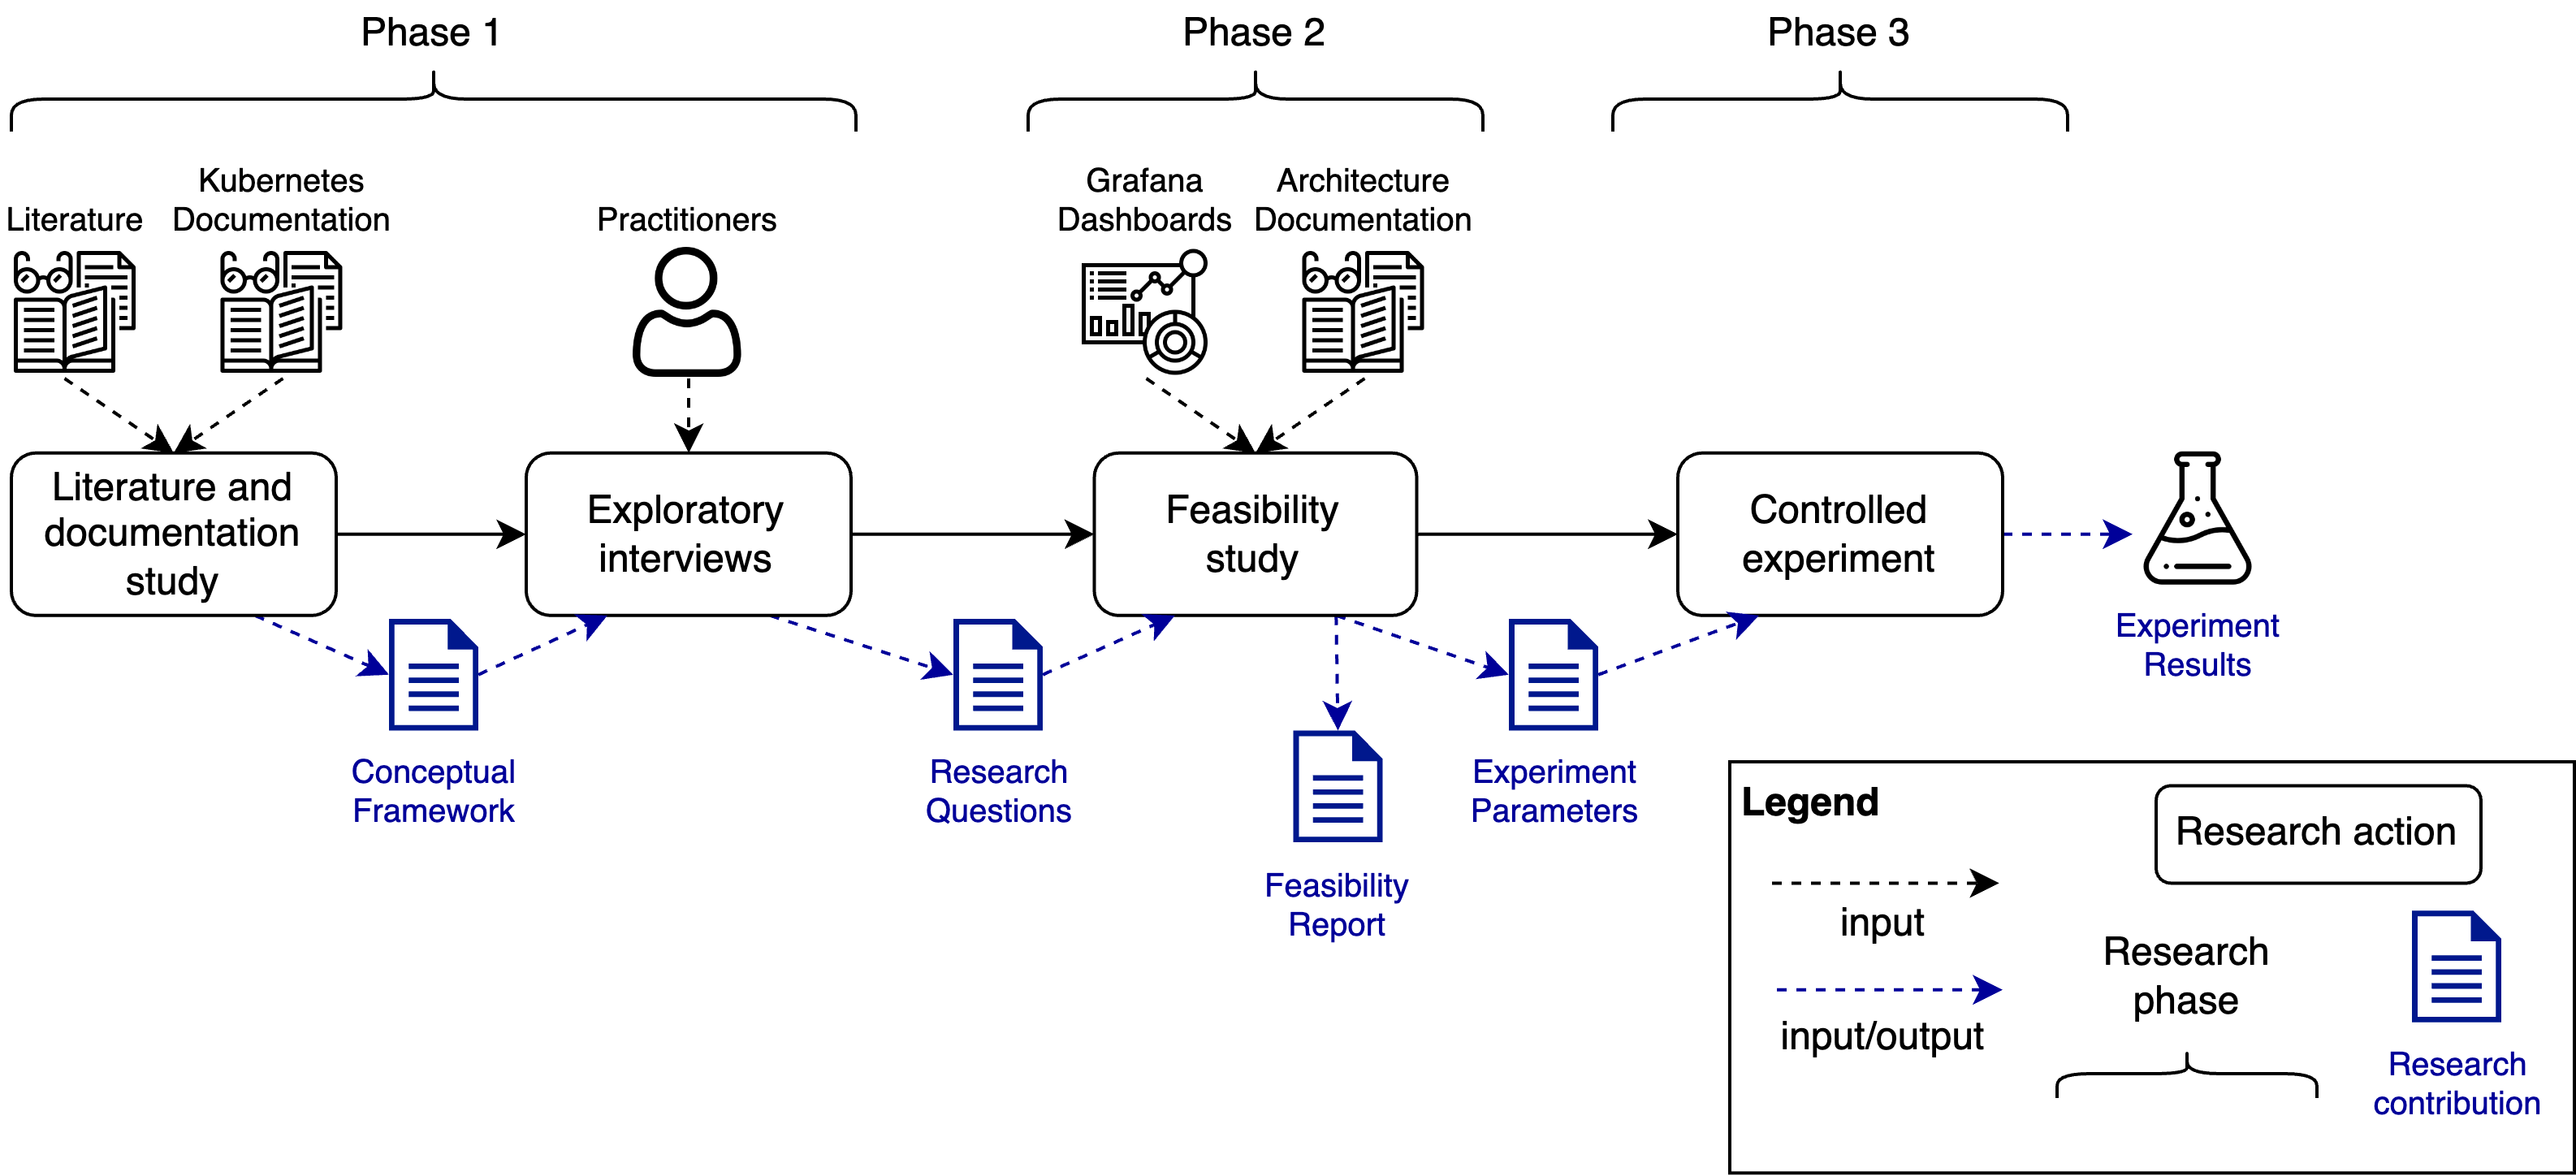
\includegraphics[width=0.9\textwidth]{figures/study-design.png}
    %% Labels should immediately follow caption, to keep latex quiet.
    \figcap{Overview: Research strategy, research methods and results. [Credits: illustration with Diagram.net]}\label{fig:method}
\end{figure*}

\lipsum[1-3]
